% !TEX TS-program = pdflatex
% !TEX encoding = UTF-8 Unicode

% This is a simple template for a LaTeX document using the "article" class.
% See "book", "report", "letter" for other types of document.

\documentclass[11pt]{article} % use larger type; default would be 10pt

\usepackage[utf8]{inputenc} % set input encoding (not needed with XeLaTeX)
\usepackage{float}

%%% Examples of Article customizations
% These packages are optional, depending whether you want the features they provide.
% See the LaTeX Companion or other references for full information.

%%% PAGE DIMENSIONS
\usepackage{geometry} % to change the page dimensions
\geometry{a4paper} % or letterpaper (US) or a5paper or....
% \geometry{margin=2in} % for example, change the margins to 2 inches all round
% \geometry{landscape} % set up the page for landscape
%   read geometry.pdf for detailed page layout information

\usepackage{graphicx} % support the \includegraphics command and options

% \usepackage[parfill]{parskip} % Activate to begin paragraphs with an empty line rather than an indent

%%% PACKAGES
\usepackage{booktabs} % for much better looking tables
\usepackage{array} % for better arrays (eg matrices) in maths
\usepackage{paralist} % very flexible & customisable lists (eg. enumerate/itemize, etc.)
\usepackage{verbatim} % adds environment for commenting out blocks of text & for better verbatim
\usepackage{subfig} % make it possible to include more than one captioned figure/table in a single float
% These packages are all incorporated in the memoir class to one degree or another...

%%% HEADERS & FOOTERS
\usepackage{fancyhdr} % This should be set AFTER setting up the page geometry
\pagestyle{fancy} % options: empty , plain , fancy
\renewcommand{\headrulewidth}{0pt} % customise the layout...
\lhead{}\chead{}\rhead{}
\lfoot{}\cfoot{\thepage}\rfoot{}

%%% SECTION TITLE APPEARANCE
\usepackage{sectsty}
\allsectionsfont{\sffamily\mdseries\upshape} % (See the fntguide.pdf for font help)
% (This matches ConTeXt defaults)

%%% ToC (table of contents) APPEARANCE
\usepackage[nottoc,notlof,notlot]{tocbibind} % Put the bibliography in the ToC
\usepackage[titles,subfigure]{tocloft} % Alter the style of the Table of Contents
\renewcommand{\cftsecfont}{\rmfamily\mdseries\upshape}
\renewcommand{\cftsecpagefont}{\rmfamily\mdseries\upshape} % No bold!

%%% END Article customizations

%%% The "real" document content comes below...

\title{Just-In-Time 3D Printing}
\author{Theodore Boyd, Lucy Campbell, James Hennessey}
\date{} % Activate to display a given date or no date (if empty),
         % otherwise the current date is printed 

\begin{document}
\maketitle

\section{Executive Summary}
In this report we discuss the research, development and analysis of our VEIV EngD group project. The focus of this work is on the field of 3D printing, specifically looking at improving the printing experience through near to real-time error mitigation.

The first part of this report covers the wider set of ideas behind our work on how that 3D printing errors can be lessened through allowing the user to manipulate the print whilst it it taking place. We then look at the structure of our task and its progress, followed by a study of the current state of the art and a look at possible approaches in the Prior Art chapter. Here we also analyse the current 3D printing approach and pipeline which we will need to build upon.

Next, we detail our approaches to the proposed solutions in the Method section, specifically looking at the programming and surveying techniques and their respective implementations and results. This is followed by a case study based investigation of that work in our Evaluation chapter, showing what we can do that previously was not possible.
Finally, we look forward to future developments and applications opened up because of our project in Future Work, and any concluding remarks and lessons learnt in the Conclusion section.

In summary, we have found, through our combined efforts, that with this upcoming new technology of 3D printing, there are a broad range of uses and applications. As the user base widens, so increases the noticeability of the failings and drawbacks of 3D printing. There are numerous annoyances with the process that we detail and tackle, including warping of prints, extrusion failures and long preparation times.

We detail relevant research, submit questionnaires to learn from experts and amateur users alike and write a software improvement to implement a new feature to help mitigate that particular problem.

At the end, we analyse the overall 3D print workflow and the features we have added along the pipeline, evaluating whether and how much we have improved the situation, through time saving or otherwise. We conclude that while 3D printing is still a fairly error-prone process, we have added substantially new features to the software that make the task more convenient.




\section{Introduction}
\subsection{Project Proposal}
The objective of this project was to advance the state-of-the-art of 3D printing. In particular the goal was to find ways to interact with and control a 3D printer `just-in-time'. Just-in-time refers to being able to control the commands sent to the printer just before they are about to be interpreted and executed by the printer. The just-in-time period is not fixed as the printer is continuously printing the object, building it up layer upon layer as is typical in all additive manufacturing. The kinds of interaction and control remained open to be influenced by the discoveries of the group as the project evolved and new discoveries were made.

The group explored the impact that just-in-time control might have on the diverse applications of 3D printing technology. The group has engaged in a dialogue with 3D print users and investigated the context within which 3D printing is emerging. 

The key principle that guided the software development process was to harness the existing software design patterns in the already open-sourced software, trying to work at a higher-level of abstractions, rather than low-level code. For example we wanted to avoid working on the firmware on the 3D printer. For a short period, we did explore the printer's firmware, to discover how feasible programming it might be and found it to be somewhat opaque and obtuse. Whilst raw access to the printer could have been useful, we deemed direct physical motor control and serial communication management as outside the scope of our project.

A second guiding principle of the project was that the software developed should remain open-source. ``Open-source is an approach to design, development, and distribution offering practical accessibility to a product's source''~\ref{reference:1}. This approach was partly taken because the 3D printers used in the project are built using open-source hardware (OSH) and operated using open-source software (OSS). The software used in the project was Cura, which is particular to the Ultimaker 3D print machines --- also used throughout. Cura and Ultimaker are one set of open-source 3D print technologies, existing alongside for example ReplicatorG software which controls, amongst other printers, the Makerbot range, all of which act upon Arduino microcontroller boards (pieces of open-source hardware found at the source of many open-source hardware devices today)~\ref{reference:1}. 

The final guiding principle in our project was to focus more heavily on expert users by not developing novice user interfaces. This decision was made slightly after the start of the project, in light of the initial gains made in the software development process leading to a more detailed understanding of the kind of control and interaction possible. 

Interviews and surveys were conducted in order to establish the wider context of the project's stakeholder groups in a landscape of existing 3D print technology capabilities, the needs of expert print users as well as some novice users, potential applications and relevant contemporary academic research.  

There were many unknown elements as to how far the group might be able to develop the just-in-time capabilities of a 3D printer. Ideas began broad and included a host of possible avenues for both applications and software development, gradually becoming more focused and specialised as the project unfolded, continuously guided by the overarching principles outlined above. The group maintained an exploratory approach throughout, creating stage deliverables as the project unfolded. 




\subsection{Project Structure}
We were a self-managed group, with internally negotiated roles and planning development decided through weekly meetings. Further monthly meetings were held with our academic supervisor Prof. Anthony Steed, to reflect upon progress and to discuss next steps.  In accordance with the recommendations of the academic supervisor the group maintained an online record of all group project materials using Google Groups and Google Docs. 

The project was chosen by the group from a number of others presented by academic staff and students to the entire VEIV 2014 class on the 6\textsuperscript{th} of November. Anthony Steed set forth the idea as a way for a group to explore 3D printing and potential for real-time haptic control. The group, who had already formed by this stage chose Anthony's idea largely to pursue a shared interest in 3D printing and as an opportunity to diversify from their thesis topics. 

The group member responsibilities were:
\begin{itemize}
\item Project management: Lucy
\item Software Development: James
\item Software Development: Theo
\end{itemize}

The project time frame was nine months. The project deliverables were set in collaboration with our supervisor and evolved alongside our understanding of both the software and 3D printing as a phenomena. The project timeline was as follows, starting in 2013 ending in 2014:

\begin{itemize}
\item Late October the group first formed. 
\item Early November projects suggestions were discussed and the idea chosen 
\item November 26\textsuperscript{th} progress report with Anthony 
\item December 27\textsuperscript{th} internal group presentation of summary of progress 
\item January 7\textsuperscript{th} next steps set forth and agreed by group.
\item February 4 \textsuperscript{th} group presented informally to the rest of VEIV cohort 
\item June 20\textsuperscript{th} first draft of report 
\item July 1\textsuperscript{st} project presented to the exam board
\item July 4\textsuperscript{th} project report submission deadline 
\item First week after Easter final report and presentation (may be presented before a public audience)
\item Regular weekly meetings were held throughout. 
\end{itemize}

The requirements of this project are therefore set to ensure group members come from across more than one academic department. In this project for example members came from schools of architecture and computer science, with expertise ranging for example from front end software development to machine learning to mathematics to service and estates management. 

This VEIV project is an interdisciplinary project~\ref{reference:4},~\ref{reference:7}. As is often the case with software development groups in the commercial world and knowledge working practices this group was a one off formation~\ref{reference:9}. The VEIV school has facilitated the project in a number of ways: first enabling access to academic expertise and leadership in the form of a project supervisor, secondly providing desk space to work together as a group, thirdly giving access to resources such as 3D printers and print materials, fourthly by allocating time in our academic schedules to produce the project and finally there will be structured criticism and feedback to prepare individuals in the group for similar future experiences. The project acted as an opportunity to reflect upon how best to bring together and work within groups of people with disparate academic experience in one off situations and produce tangible outcomes, a subject of current focus in UCL and the wider academic community~\ref{reference:5},~\ref{reference:6},~\ref{reference:8},~\ref{reference:10}. 

The associated academic faculties of this project, from which resources were provided via the VEIV program structure, were Computer Science (where the VEIV school staff and students reside in large part), the Make Space which is a cross departmental workshop space providing materials and equipment such as 3D printers as well as technical support, and finally the Bartlett faculty of the Built Environment who supported our project to a smaller extent, providing secondary academic support and meeting spaces (also where a further cohort of the VEIV school reside).

The support that is mentioned above was effective in facilitating team working in the project, in particular the group found that having physical space to work together facilitated understanding of new concepts presented by members in light of their different academic backgrounds. The academic leadership gave the group focus, greater access to physical resources which was essential in progressing our work. The structural guidelines set forth by the VEIV school were also invaluable. Ours was a small group, formed prior to choosing a project to work on, we felt that these were positive factors in the project, giving us greater cohesion and control of the project. 

We openly shared ideas within the group as well as with the wider 3D print community, communicating on online forums and through surveys. Our group embraced the structure of the VEIV project as an opportunity to collaborate openly and work in a team, to increase the accessibility and generalisability of our work using broader methods and more accessible language to record and communicate our work~\ref{reference:5},~\ref{reference:6}. 

We chose to work on OSS as the machines that we used operate on OSS. The group sought guidance about Cura from within the existing code itself and via online discussion forums. There is little formal documentation and guidance about the development of Cura, a common, well-accepted challenge when developing OSS~\ref{reference:11}~\ref{reference:60}. Using OSS was an opportunity to make a direct contribution to a community of developers who will hopefully build upon the innovations of just-in-time control~\ref{reference:12},~\ref{reference:67}. 





\subsection{Motivation}
Our group was delighted to have an opportunity to work in such an active field of research. 3D printing is a phenomenon that captures widespread attention at many levels of society around the world, it is the source of much anticipated opportunity for economic success and has generated a seemingly exponentially growing industry~\ref{reference:13}. Associated research about 3D printing has been complimentarily intense and the potential applications are wide ranging and continuously evolving~\ref{reference:17}. 

One of the overarching ideologies emerging from the barrage of developments in 3D printing is that manufacturing and product development are now increasingly happening from the bottom up, with individuals able to print any object within their price range and within the receding limitations of the technology available from home~\ref{reference:13}. It has been speculated that 3D printing will change the integral nature of manufacturing along with the associated logistical and production processes involved, as people gain the ability to manufacture at the at the user's location~\ref{reference:16}. Anxiety has arisen over the accessibility of 3D printing and its potential applications, fuelled by media stories for example about 3D printed guns~\ref{reference:15}. Regulation, design patents and copyrights on 3D printed objects may therefore have an increasing impact~\ref{reference:13}. While the regulatory aspects of 3D printing may seem unrelated currently, such matters may be a growing consideration in any resultant applications of our project. To name an example, if a design was patented and our new system then reproduced an altered that design, would it belong to us or to the original designer?

Although the potential of 3D printing is vast, there remains much research and development work still to be done to improve the quality of the technologies and software available, to make them more accessible to a wider set of users and capable of creating more complex objects. There are persistent limitations to 3D print technologies, for example the “stair-stepping” effect of fused deposition model (FDM) technologies, explained in more detail in section \ref{section:TechnologyLandscape} of the report, whereby ‘parts cannot accurately conform to the CAD geometry in the vertical plane’~\ref{reference:18}. This was reported in~\ref{reference:44} and was reiterated last year by Nannan and Ming in their paper on Additive manufacturing: technology, applications and research needs~\ref{reference:17},~\ref{reference:18}. 

3D printing processes are unreliable across the spectrum of the different kinds of technologies available for different reasons. While failure rate increases in the lower costing 3D print machines such as the Ultimaker and RepRap, failures become more costly in higher end commercial machines where occurrences are fewer, however waste more time and potentially finite and costly materials as well as causing wear and tear to the machines themselves. Given the widespread and impeding level of errors encountered in 3D printing technologies, this was a most compelling motivation for our project and a central objective of our group was to apply just-in-time control of a 3D printer to solve recurring errors. 

One cross section of 3D print users who we were particularly interested in and who commonly use the same machines available to us throughout our project can loosely be described as the ‘maker’ community. While the trend of making is broader than 3D printing alone, groups are utilising the technology and incorporate open software and hardware technologies such as Arduino and Cura in their work. ‘The availability of low-cost machines allowed other projects to start, inspired the 'makers' movement, helped the diffusion of fablabs and prototyping boards such as the Arduino, and it even started an economy’~\ref{reference:19}. Some examples of maker community groups who utilise similar technologies to us are the HackSpace or Makerverse who are resident in London or attendees of the MakerFair conference events, who are strongly linked to academic research and institutions as well~\ref{reference:14}. We feel that these groups share our project ethos of exploring accessible technologies for people to use to aid innovation. 

As our group work uses similar technology and has a similar outlook as the maker community our project has an inherent strong link to the creative and generate innovative applications being explored. It was therefore natural that we consider how the just in time capabilities that we developed might also benefit the lineage of designers and artists using 3D printing.  

Even though we are motivated by the types of work happening in maker communities, by contemporary research and by applications in design, the problem of errors occurring in the 3D printing process is overarching and much of our work has been informed by contemporary academic research, discussed in the section of this report entitled Current Approaches, as well as by discussions with commercial 3D print users. We were unable in the given timeframe to address all potential applications of ‘just in time’ control, for example commercial application of our project as a design tool would require a more robust investigation of user interfaces, and there are a plethora of industries actively researching 3D printing such as aerospace, transport or fashion not discussed here.





\section{Prior Art}
\subsection{Technology Landscape}
\label{section:TechnologyLandscape}
While our project used an Ultimaker FDM printer, there are a number of ways to produce a three-dimensional physical object using machinery. They usually fall into either additive or subtractive techniques. Before the advent of modern technologies, additive techniques were based around pouring materials into moulds and subtractive techniques used tools such as chisels and lathes to sculpt larger blocks of raw material into the final output~\ref{reference:23}.

In recent decades, we have seen a new innovation in the form of three-dimensional object production using automation and information technology (IT). Automation involves both mechanisation and industrialisation of techniques, while the use of IT allows for computerised systems to pre-program parameters, batch processing jobs and ease repetitive or high-volume tasks.

New technologies have opened up new subtractive forms. They include for example computer numerical control (CNC) mills and routers. The additive form is that associated with the field of 3D printing~\ref{reference:20}. 

Additive manufacturing (AM) is today synonymous with 3D printing\footnote{However, in the literature, the terms did not traditionally cover the same fields.} and it has become an ever more popular and useful technique with a growing number of applications and a shrinking of price points~\ref{reference:27}. AM can take a number of forms~\ref{reference:23} but is broadly defined as a collection of computer-controlled processes of creating parts in a layerwise fashion, that is joining of a layer of material onto layers laid down or cured previously, without part-specific tooling~\ref{reference:34}. A reference definition is provided by the American Society for Testing and Materials (~\ref{reference:59}, ASTM) as ASTM F2792–10. Subtractive forms of manufacture are more traditional and there is general agreement amongst those using the technology, that additive forms can work with increased accuracy, precision and resolution~\ref{reference:26}.

Availability of 3D computer models was crucial to realising the concept of layered object creation, but other technologies such as affordable laser systems, photocurable materials, and powerful personal computers helped to disseminate this technology as well~\ref{reference:24}. Critical enabling developments included the advent of desktop computers and the economic development and availability of industrial lasers~\ref{reference:25}.

Forms of AM include the use of heated extrusion of materials (especially thermoplastics but also rubber) known as fused deposition modelling (FDM). FDM is particularly popular due to the relatively low cost of materials and high commercial potential easing its spread into the non-professional market from AM's origins as a professional tool. We shall cover FDM in more detail later as it is the format our printer used. The printer we have chosen is the Ultimaker - low specification machines such as the Ultimaker can retail at under £1,000~\ref{reference:28} and previous models such as the Reprap have even been specifically designed to be self replicating, inherently widening their accessibility, see Figure~\ref{figure:FDM}.

\begin{figure}[H]
  \centering
  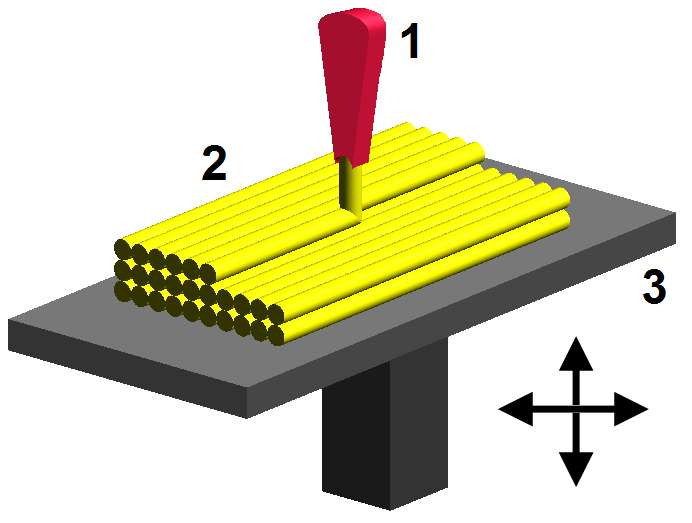
\includegraphics[width=4in]{FDM_by_Zureks.png}
  \caption{Fused deposition modelling schematic~\ref{reference:35}}
  \label{figure:FDM}
\end{figure}

Other AM processes use beams of electrons or photons (lasers) to create pools of molten metals, known as Electron Beam Freeform Fabrication (EBF3) or if not melting it completely, sintering. For powdered metals and other granular materials, there is also a similar process called Direct Metal Laser Sintering (DMLS) and its variants~\ref{reference:29}.

For more challenging materials than metals and plastics, more complex techniques have been developed. For plaster, binder can be printed onto the particles using an inkjet head (similar to those used in standard 2D printing) to selectively bind particles from a larger powder bed~\ref{reference:30}. For paper and films made of plastics and metals, Laminated Object Manufacturing (LOM) uses a laser beam to cut out the current layer's shape before the film rollers roll out a new layer on top to cut~\ref{reference:31}.

It is also possible to use light sensitive chemicals for an approach that allows for construction not constrained by the printer rig's dimensions. Known as photopolymerisation or stereolithography, this approach solidifies, or cures, a light-sensitive material such as a gel or liquid, by applying light beams to locations in a bath of the material that are to be part of the object, leaving the remainder uncured and reusable. Through the raising or lowering of the laser or bath, layers can be constructed in a similar fashion to more standard, dry methods of additive manufacturing. A variant, Mask Projection Stereolithography (MPS) machine projects a light beam mask over the material bath surface to protect the material that does not need to be cured~\ref{reference:33}, see Figure~\ref{figure:SLA}.

\begin{figure}[H]
  \centering
  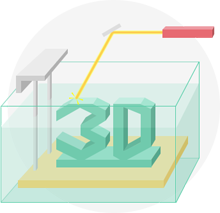
\includegraphics[width=4in]{sla.png}
  \caption{Photopolymerisation~\ref{reference:32}}
  \label{figure:SLA}
\end{figure}

With the recent consumerisation of fused deposition modelling, this method of 3D printing has received a large amount of coverage and usage in recent years. It is an important area of growth with a very broad range of uses, reaching into art and design as well as manufacturing, construction and prototyping. Initially only a professional's tool, FDM and AM as a whole is now accessible to many hobbyists, proving its worth in society as a hacker's or maker's tool mentioned previously, drawing many similarities to the initial growth of the personal computer market at the end of the last millennium~\ref{reference:21},~\ref{reference:22}.

A widening audience has also brought to light a number of problems with the nascent technology. And so we have found now to be the opportune time to experiment with, and attempt to solve, a number of these as it is of utmost importance that this technology grow and be further explored to perhaps give it the chance that the personal computer was given previously.

Whilst all of additive manufacturing is very applicable today, FDM in particular is a very promising new technology for wide distribution, and so it would be particularly beneficial to the fabrication community as a whole to address the most frequent hurdles encountered in it. It also gives us the chance to focus our efforts on one of the more popular modes of AM, reaching the widest popular audience whilst still being able to produce targeted solutions that are not too diluted by abstraction to the variants of AM.




\subsection{Current Approaches}
This section discusses work being done in recent years, that shares common characteristics with our project. Much of the work discussed is focused on prototyping processes, ranging from rapid tooling engineering to medical prototyping~\ref{reference:42},~\ref{reference:44}. 

There are a number of projects which analyse 3D models before printing them, to calculate the correct geometries of a shape for some particular set of optimisations and alter it accordingly through a series of algorithmic equations. The project Make It Stand: Balancing Shapes for 3D Fabrication made it possible to interactively deform an existing model, pre-empting print failures by altering the mesh of the model. Researchers addressed the problem of how to balance a 3D model, as often a printed object would be weighted incorrectly because of overhangs and the centre of mass makes it unbalanced~\ref{reference:36}. The project applies an algorithm to manually carve and deform a model using the initial surface mesh as an input and relaying back to the user who manually alters the model until it is optimally positioned, sized and weighted to ‘stand up’. 

The project, Making Burr Puzzles from 3D Models optimises and arranges the orientation of a model in the pre-processing phase, splitting complex 3D shapes into puzzle pieces automatically~\ref{reference:43}. Others have updated the model to strengthen the object being printed, redistributing mass where points are particularly thin for example~\ref{reference:45}. Such projects achieve ‘structural analysis on the user side which, with conventional tools is often infeasible as it requires specialised training and software. ‘Trial-and-error, the most common approach, is time-consuming and expensive’~\ref{reference:46}. 

In Selective laser sintering (SLS) printing techniques there is active research into how the level of errors incurred can be mitigated, although Tang et al. argue more generally that it is impossible to achieve perfection in AM techniques~\ref{reference:37}. One of the central drives for improving outcomes, in part comes from the potential to use SLS processes in medical research, for example to fabricate prototypes from biomedical images in maxillofacial surgery procedures~\ref{reference:38},~\ref{reference:39}. Research papers focusing on this particular application analyse the accuracy and reliability of SLS processes~\ref{reference:38},~\ref{reference:39}, however the solutions offered are limited, finding errors through trial and error or improving upon this by calculating for errors in the pre-processing phase, similar to the examples mentioned above. This inherently means that the user must know the potential errors and or abort the print job once it has begun. This is particularly wasteful in scenarios when the print time extends over several hours, after which the user returns to find the failed print, wasting materials and time. 

Current related projects work at the pre-processing phase in comparison to our project which deals with the manufacture stage, although they do focus on foreseeing and mitigating errors. 

In the context of work being done to improve reliability of different industrial manufacturing processes, there has been some breakthrough in automating feedback about the object once manufacture has begun, using sensors and an understanding of different kinds of shape optimisation. Improvements to the machinery itself and reliability of materials are often a central focus in contrast to the examples above, which focus heavily on areas of high level programming~\ref{reference:37}. In research by Shin et al. into Layered Manufacturing (also referred to as Solid Freeform Fabrication), they introduce feedback loops to the manufacture process in the form of sensors and a camera, in order to alter an object as it is being produced.

\begin{figure}[H]
  \centering
  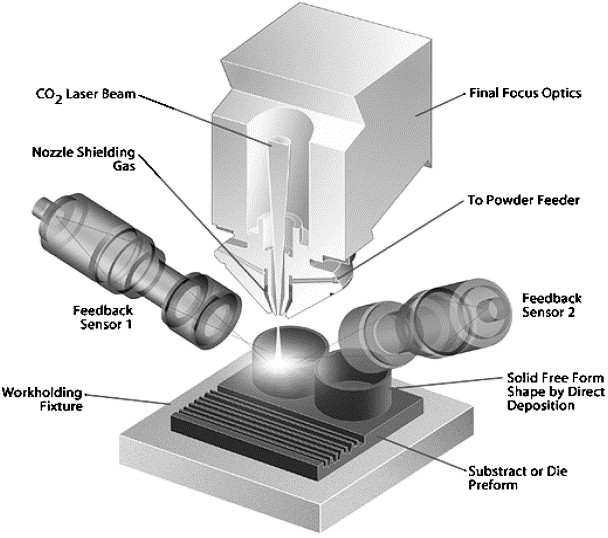
\includegraphics[width=4in]{shin.jpg}
  \caption{Direct metal deposition layered manufacturing system~\ref{reference:40}}
  \label{figure:Shin}
\end{figure}

The image in Figure~\ref{figure:Shin} shows that based on the material properties of the object the optimal density can be calculated in relation to specific stress points while the manufacture is taking place, to make changes in the materials during the print process~\ref{reference:40},~\ref{reference:41}. The process of change happens as the material is being extruded. The developments made by the research groups above brings the alteration process into the manufacture phase in a similar way to our project and further is able to incorporate information about the already printed parts of the object.  

In sum, rapid prototyping is becoming more or less standard in product development and a second wave of technological creativity is finding its way to industrial practise. The approaches mentioned above are set apart from our research as we are exploring new interesting areas, after the printing process has already begun coupled with more widely available low-cost FDM print technology. 


\subsection{Pre-Existing Pipeline}




\section{Method}
\subsection{Surveys}


\subsection{Buffer Control}



\subsection{G-code Manipulation}



\subsection{Improved Duration Estimation}



\subsection{Parameter Adjustments}



\subsection{Adaptive Skirt}



\subsection{Geometry Manipulation}



\section{Evaluation}
\subsection{Results}




\section{Future Work}
\subsection{Improved Geometry Manipulation}




\subsection{Automated Error Mitigation}




\subsection{Design Tool}




\section{Conclusion}

\subsection{Buffer Control}


% Bibliography
\nocite{*}
\bibliographystyle{plain}
\bibliography{bibliogVer1}

\end{document}
